\subsection{Tabelas}

\begin{frame}
\frametitle{Tabelas}
Tabelas convêm informação em forma visual.

%Uma tabela é um arranjo de células organizadas em colunas verticais e linhas horizontais.
%As células são elementos mínimos indivisíveis. Dependendo da necessidade, as células podem
%ser mescadas, expandindo assim ao longo de linhas (\verb|\multirow|) ou colunas (\verb|\multicolumn|). 
\vspace{9ex}

\centering
\begin{tabular}{ l c r }
  1 & 2 & 3 \\
  4 & 5 & 6 \\
  7 & 8 & 9 \\
\end{tabular}
\end{frame}


\begin{frame}
\frametitle{Utilize tabelas apenas quando necessário}
\begin{table}[h]
\caption{\label{tab-receita}Receita Coffee Porter (OG: 1,055, FG: 1,012, ABV: 5,6\%, COR: 40, IBU: 27).}
\begin{tabular}{|l|l|l|}
\hline
	& quantidade & ingrediente \\
\hline
\multirow{4}{*}{brassagem} & 3,0 kg & Dry Brew Extrato de Malte \\
	& 0,5 kg & Malte Cara Gold \\
	& 0,4 kg & Malte Chocolate \\
	& 0,3kg & Cevada Torrada \\
\hline 
\multirow{2}{*}{Fervura} & 25g & Target @30min \\
	& 20g & Fuggles @15min \\
\hline
\multirow{2}{*}{Fermentação} & \multirow{2}{*}{1} & Levedura Levteck American Ale \\
	& & 10 dias @ 18C, 7 dias @ 5C \\
\hline
\multirow{2}{*}{envase} & 300ml & Café \\
	&  5g/L & primming \\
\hline
\end{tabular}
\end{table}
\end{frame}

\begin{frame}
\frametitle{Utilize tabelas apenas quando necessário}
\textbf{Receita Coffee Porter}

{\small características: \\OG: 1,055, FG: 1,012, ABV: 5,6\%, COR: 40, IBU: 27}
\begin{description}
\item[brassagem] 
	\begin{itemize}
	\item[--] 3,0 kg Dry Brew Extrato de Malte
	\item[--] 0,5 kg Malte Cara Gold
	\item[--] 0,4 kg Malte Chocolate
	\item[--] 0,3kg Cevada Torrada
	\end{itemize}
\item[fervura]
	\begin{itemize}
	\item[--] 25g Target @30min
	\item[--] 20g Fuggles @15min
	\end{itemize}
\item[fermentação]
	\begin{itemize}
	\item[--] Levedura Levteck American Ale - 10 dias @ 18C, 7 dias @ 5C
	\end{itemize}
\item[envase]
	\begin{itemize}
	\item[--] 300ml de Café
	\item[--] primming: 5g/L
	\end{itemize}
\end{description}
\end{frame}


\begin{frame}[fragile,allowframebreaks]
\frametitle{Tabelas em \LaTeX{}}
\begin{lstlisting}[language=tex, label=lst-tabela, caption={Exemplo de documento em \LaTeX{}}, postbreak=\mbox{$\hookrightarrow$\space}, basicstyle=\fontsize{8}{10}\selectfont\ttfamily]
\begin{tabular}{ l c r }
  1 & 2 & 3 \\
  4 & 5 & 6 \\
  7 & 8 & 9 \\
\end{tabular}
\end{lstlisting}

Definição: \verb|\begin{tabular}[pos]{table spec}|

Onde \texttt{table spec} especifica o alinhamento de cada coluna.

\begin{description}
\item[l] esquerda (\emph{left})
\item[c] centralizado (\emph{centered})
\item[r] direita (\emph{right})
\item[p] parágrafo, deve-se utilizar a sintaxe \verb|p{'width'}| (\emph{paragraph}) 
\item[|] linha vertical
\end{description}

\vspace{3ex}
Definição de múltiplas colunas: \verb|*{num}{str}|

Exemplo: \verb|\begin{tabular}{l*{6}{c}r}|

\framebreak

\vspace{3ex}
Células podem ser mescladas: \verb|\multirow| ou \verb|\multicolumn|.


Sintaxe do comando \verb|\multicolumn|: \\
\verb|\multicolumn{num_cols}{alignment}{contents}|

\begin{description}
\item[num\_cols] número de colunas subsequentes que serão mescladas
\item[alignment] opções de alinhamento \texttt{l, c, r, p}
\item[contents] conteúdo da célula
\end{description}

\framebreak

Sintaxe do comando \verb|\multirow|: \\
\verb|\multirow{num_rows}{width}{contents}|

\begin{description}
\item[num\_rows] número de linhas que serão mescladas
\item[width] largura do texto. O valor \texttt{*} indica a largura natural e \texttt{=} indica a largura da coluna
\end{description}

\end{frame}


\begin{frame}[allowframebreaks,fragile]
\frametitle{Células de múltiplas colunas}

\lstinputlisting[language=tex, label=lst-ex-multicols, postbreak=\mbox{$\hookrightarrow$\space}, basicstyle=\fontsize{8}{10}\selectfont\ttfamily]{examples/multicol.tex}
\begin{table}[ht]
\caption{Multi-column table}
\begin{center}
\begin{tabular}{cc}
    \hline
    \multicolumn{2}{c}{Multi-column}\\
    X&X\\
    \hline
\end{tabular}
\end{center}
\label{tab:multicol}
\end{table}


\end{frame}

\begin{frame}[allowframebreaks,fragile]
\frametitle{Células de múltiplas linhas}

\lstinputlisting[language=tex, label=lst-ex-multicols, postbreak=\mbox{$\hookrightarrow$\space}, basicstyle=\fontsize{8}{10}\selectfont\ttfamily]{examples/multirow.tex}
%\usepackage{multirow} % include in document preamble
\begin{table}[ht]
\caption{Multi-row table}
\begin{center}
\begin{tabular}{cc}
    \hline
    \multirow{2}{*}{Multirow}&X\\
    &X\\
    \hline
\end{tabular}
\end{center}
\label{tab:multicol}
\end{table}


\end{frame}





\begin{frame}
\frametitle{Tabelas}
\centering
\scriptsize
\begin{table}[h]
\csvreader[tabular=|l|l|,
    table head=\hline \bfseries mês & \bfseries gás (R\$),
    late after head=\\\hline\hline,
    late after line=\\\hline,
    filter={\value{csvrow}<18},
    ]%
    {/home/leoca/docs/ape/lodz/consumo/consumo.csv}%
    {mes=\mes,gas=\gas}% use head of csv as column names
    {\mes & \gas}% specify your coloumns here
\caption{\label{tab-example01}Valor gasto mensalmente com gás.}
\end{table}
\end{frame}

\begin{frame}
\frametitle{Tabelas}
\centering
\scriptsize
\begin{table}[h]
\csvreader[tabular=|l|l|,
    before table=\rowcolors{2}{red!25}{yellow!50},
    table head=\hline\rowcolor{red!50!black}\color{white}\bfseries mês & \color{white}\bfseries gás (R\$),
    late after head=\\\hline\hline,
    late after last line=\\\hline,
    filter={\value{csvrow}<18},
    ]%
    {/home/leoca/docs/ape/lodz/consumo/consumo.csv}%
    {mes=\mes,gas=\gas}% use head of csv as column names
    {\mes & \gas}% specify your coloumns here
\caption{\label{tab-example02}Valor gasto mensalmente com gás.}
\end{table}
\end{frame}



\begin{frame}
\frametitle{Tabelas}
\centering
\scriptsize
\begin{table}[h]
\csvstyle{mystyle}{
    tabular=lH,
    head to column names,
    table head=\toprule {mês} & {gás (R\$)} \\\midrule,
    table foot=\bottomrule,
    filter={\value{csvrow}<18}
}
\csvreader[mystyle]{/home/leoca/docs/ape/lodz/consumo/consumo.csv}{}{\mes & \gas}
\caption{\label{tab-example03}Valor gasto mensalmente com gás.}
\end{table}
\end{frame}

\begin{frame}[fragile]
\frametitle{Código utilizado na tabela anterior}
\begin{lstlisting}[language=tex, label=lst-tabela, caption={Tabela gerada a partir de um arquivo CSV. Pacotes utilizados: csvsimple e booktabs.}, postbreak=\mbox{$\hookrightarrow$\space}, basicstyle=\fontsize{8}{10}\selectfont\ttfamily]
\csvstyle{mystyle}{
    tabular=lH,
    head to column names,
    table head=\toprule {mês} & {gás (R\$)} \\\midrule,
    table foot=\bottomrule,
    filter={\value{csvrow}<18}
}
\csvreader[mystyle]{consumo.csv}{}{\mes & \gas}
\end{lstlisting}
\end{frame}


\begin{frame}
\frametitle{Tabelas}
\centering
\scriptsize
\begin{table}[h]
\csvstyle{mystyle}{
    tabular=lH,
    head to column names,
    table head= {mês} & {gás (R\$)} \\\midrule,
    filter={\value{csvrow}<18}
}
\csvreader[mystyle]{/home/leoca/docs/ape/lodz/consumo/consumo.csv}{}{\mes & \gas}
\caption{\label{tab-example03}Valor gasto mensalmente com gás.}
\end{table}
\end{frame}



\begin{frame}
\frametitle{Comparação entre duas tabelas}
\begin{figure}[htbp]
\begin{minipage}[t]{0.47\textwidth}
\centering
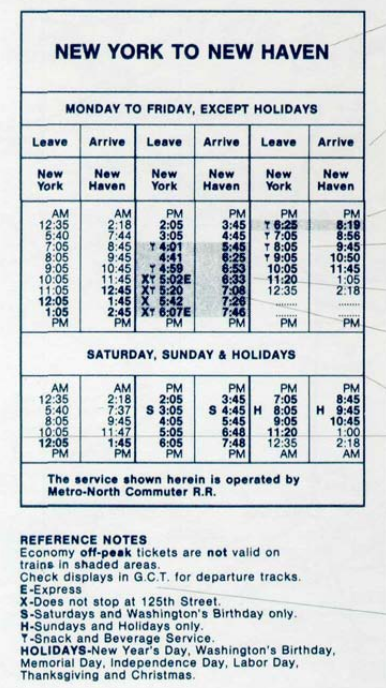
\includegraphics[width=0.64\linewidth,height=0.7\textheight,keepaspectratio]{figures/timetable01.png}
\subcaption{Design ruim.}
\end{minipage}
\hfill
\begin{minipage}[t]{0.47\textwidth}
\centering
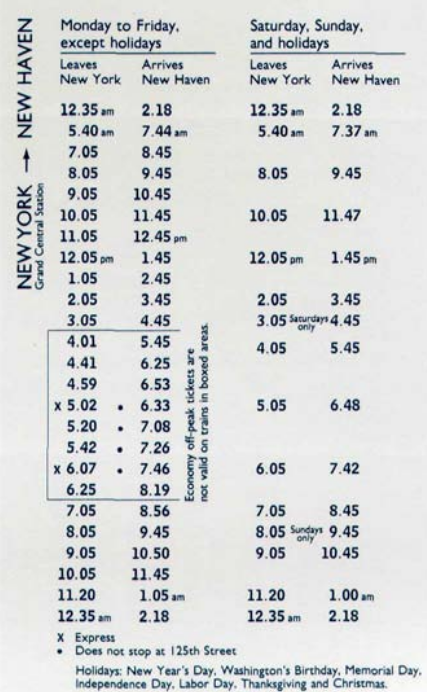
\includegraphics[width=0.7\linewidth,height=0.7\textheight,keepaspectratio]{figures/timetable02.png}
\subcaption{Bom design.}
\end{minipage}
\caption{Tabelas com horários do trem \cite{tufte_envisioning_1990}.}
\end{figure}
% pg105 - Envisioning Information, Edward R. Tufte
% bad design: 
% - direction of the train is not clear
% - repeated headings
% - zig-zag reading
% - poor usege of empty spaces
\end{frame}

\begin{frame}[fragile,allowframebreaks]
\frametitle{stargazer (R)}
\framesubtitle{\emph{Well-Formatted Regression and Summary Statistics Tables}}

\emph{stargazer} é um pacote em R para produzir tabelas bem formatadas em \LaTeX{},
HTML/CSS e ASCII.

\url{https://cran.r-project.org/web/packages/stargazer/}


\begin{lstlisting}[language=R, label=lst-stargazer, caption={Exemplos de utilização do stargazer}, postbreak=\mbox{$\hookrightarrow$\space}, basicstyle=\fontsize{8}{10}\selectfont\ttfamily]
library(stargazer)
stargazer(attitude)
\end{lstlisting}

O resultado é exibido na listagem \ref{lst-ex-stargazer} e na tabela \ref{tab-ex-stargazer}.

\lstinputlisting[language=tex, label=lst-ex-stargazer, postbreak=\mbox{$\hookrightarrow$\space}, basicstyle=\fontsize{8}{10}\selectfont\ttfamily]{ex-stargazer.tex}

\framebreak
\begin{table}[!htbp] \centering 
  \caption{Exemplo gerado pelo \texttt{stargazer} usando o dataframe \texttt{attitude}.} 
  \label{tab-ex-stargazer} 
\begin{tabular}{@{\extracolsep{5pt}}lccccccc} 
\\[-1.8ex]\hline 
\hline \\[-1.8ex] 
Statistic & \multicolumn{1}{c}{N} & \multicolumn{1}{c}{Mean} & \multicolumn{1}{c}{St. Dev.} & \multicolumn{1}{c}{Min} & \multicolumn{1}{c}{Pctl(25)} & \multicolumn{1}{c}{Pctl(75)} & \multicolumn{1}{c}{Max} \\ 
\hline \\[-1.8ex] 
rating & 30 & 64.633 & 12.173 & 40 & 58.8 & 71.8 & 85 \\ 
complaints & 30 & 66.600 & 13.315 & 37 & 58.5 & 77 & 90 \\ 
privileges & 30 & 53.133 & 12.235 & 30 & 45 & 62.5 & 83 \\ 
learning & 30 & 56.367 & 11.737 & 34 & 47 & 66.8 & 75 \\ 
raises & 30 & 64.633 & 10.397 & 43 & 58.2 & 71 & 88 \\ 
critical & 30 & 74.767 & 9.895 & 49 & 69.2 & 80 & 92 \\ 
advance & 30 & 42.933 & 10.289 & 25 & 35 & 47.8 & 72 \\ 
\hline \\[-1.8ex] 
\end{tabular} 
\end{table} 



\end{frame}


\begin{frame}[fragile,allowframebreaks]
\frametitle{Octave to \LaTeX{}}

\begin{lstlisting}[language=Octave, label=lst-octave-matrix, caption={Gerando a matriz em \LaTeX{} a partir do GNU Octave}, postbreak=\mbox{$\hookrightarrow$\space}, basicstyle=\fontsize{8}{10}\selectfont\ttfamily]
A = magic(8);
strcat("\\begin{bmatrix}\n",strrep(strrep(mat2str(A)," "," & "),";","\\\\\n")(2:end-1),"\n\\end{bmatrix}\n")
\end{lstlisting}

$
\begin{bmatrix}
64 & 2 & 3 & 61 & 60 & 6 & 7 & 57\\
9 & 55 & 54 & 12 & 13 & 51 & 50 & 16\\
17 & 47 & 46 & 20 & 21 & 43 & 42 & 24\\
40 & 26 & 27 & 37 & 36 & 30 & 31 & 33\\
32 & 34 & 35 & 29 & 28 & 38 & 39 & 25\\
41 & 23 & 22 & 44 & 45 & 19 & 18 & 48\\
49 & 15 & 14 & 52 & 53 & 11 & 10 & 56\\
8 & 58 & 59 & 5 & 4 & 62 & 63 & 1
\end{bmatrix}

$

\begin{lstlisting}[language=Octave, label=lst-octave-table, caption={Gerando uma tabela em \LaTeX{} a partir do GNU Octave}, postbreak=\mbox{$\hookrightarrow$\space}, basicstyle=\fontsize{8}{10}\selectfont\ttfamily]
A = magic(8);
strcat("\\begin{table}[!htbp]\\centering\n\\caption{}\n\\label{}\n\\begin{tabular}{",repmat('l',1,size(A,2)),"}\n\\hline\n",strrep(strrep(mat2str(A)," "," & "),";","\\\\\n")(2:end-1),"\\\\\n\\hline\n\\end{tabular}\n\\end{table}")
\end{lstlisting}

\framebreak
\begin{table}[!htbp]\centering
\caption{Tabela gerada através do GNU Octave.}
\label{tbl-ex-octave}
\begin{tabular}{llllllll}
\hline
64 & 2 & 3 & 61 & 60 & 6 & 7 & 57\\
9 & 55 & 54 & 12 & 13 & 51 & 50 & 16\\
17 & 47 & 46 & 20 & 21 & 43 & 42 & 24\\
40 & 26 & 27 & 37 & 36 & 30 & 31 & 33\\
32 & 34 & 35 & 29 & 28 & 38 & 39 & 25\\
41 & 23 & 22 & 44 & 45 & 19 & 18 & 48\\
49 & 15 & 14 & 52 & 53 & 11 & 10 & 56\\
8 & 58 & 59 & 5 & 4 & 62 & 63 & 1\\
\hline
\end{tabular}
\end{table}


\framebreak
\lstinputlisting[language=tex, label=lst-ex-octave-table, postbreak=\mbox{$\hookrightarrow$\space}, basicstyle=\fontsize{8}{10}\selectfont\ttfamily]{examples/octave-table.tex}

\end{frame}



\begin{frame}
\frametitle{Dicas}
\begin{itemize}
\item \hrefcolor{https://www.tablesgenerator.com/}{tables generator}
\item \hrefcolor{https://www.latex-tables.com/}{latex tables}
\end{itemize}
\end{frame}




\begin{frame}
Sugestões de leitura: 
\vspace{2ex}

\hrefcolor{https://en.wikibooks.org/wiki/LaTeX/Tables}{Wikibooks - \LaTeX{} / Tables}
\vspace{2ex}

\fullcite{chicago_2017}
\end{frame}
